\chapter{Feature Engineering Details}

This appendix provides additional information on the feature engineering and data preprocessing steps that were performed to prepare the dataset for machine learning model training.

\section{Feature Transformation Methods}

Several feature transformation techniques were applied to improve the model performance and handle the characteristics of network traffic data:

\subsection{Log Transformation}

To address the highly skewed distributions common in network traffic volume metrics (bytes and packets), a logarithmic transformation was applied:

\begin{equation}
x'_i = \log(x_i + 1)
\end{equation}

The addition of 1 before taking the logarithm prevents undefined values for zero values, which are common in network flow data. This transformation was applied to the following features:
\begin{itemize}
    \item orig\_bytes
    \item resp\_bytes
    \item orig\_pkts
    \item resp\_pkts
    \item duration
\end{itemize}

\subsection{Categorical Feature Encoding}

For categorical features, the following encoding schemes were applied:

\begin{table}[h]
\centering
\caption{Categorical feature encoding methods}
\label{tab:categorical_encoding}
\begin{tabular}{lll}
\hline
\textbf{Feature} & \textbf{Encoding Method} & \textbf{Cardinality} \\
\hline
proto & One-hot encoding & 3 (TCP, UDP, ICMP) \\
conn\_state & One-hot encoding & 11 unique states \\
service & Target encoding & 30+ unique values \\
\hline
\end{tabular}
\end{table}

For the'service' feature, which had high cardinality, target encoding was used instead of one-hot encoding to avoid creating too many sparse features. The target encoding replaces each category value with the mean of the target variable for that category.

\section{Derived Features}

The table below describes the complete set of engineered features that were derived from the original dataset attributes:

\begin{table}[h]
\centering
\caption{Description of engineered features}
\label{tab:engineered_features}
\begin{tabular}{lp{10cm}}
\hline
\textbf{Feature Name} & \textbf{Description} \\
\hline
total\_bytes & Sum of bytes in both directions (orig\_bytes + resp\_bytes) \\
total\_pkts & Sum of packets in both directions (orig\_pkts + resp\_pkts) \\
bytes\_per\_pkt\_orig & Average bytes per packet in the original direction (orig\_bytes / orig\_pkts) \\
bytes\_per\_pkt\_resp & Average bytes per packet in the response direction (resp\_bytes / resp\_pkts) \\
bytes\_ratio & Ratio of original to response bytes (orig\_bytes / resp\_bytes) \\
pkts\_ratio & Ratio of original to response packets (orig\_pkts / resp\_pkts) \\
is\_backscatter & Binary indicator for potential backscatter traffic (based on connection state and protocol) \\
hour\_of\_day & Hour extracted from the timestamp (0-23) \\
is\_weekend & Binary indicator for weekend connections (1 for Saturday/Sunday) \\
conn\_rate\_5min & Connection rate within a 5-minute window for the same source IP \\
port\_scan\_score & Number of unique destination ports contacted by the same source IP within a 5-minute window \\
is\_scanning\_behavior & Binary indicator for potential scanning behavior (many connections, few bytes) \\
time\_delta\_mean & Average time between consecutive connections from the same source IP \\
time\_delta\_std & Standard deviation of time between consecutive connections from the same source IP \\
\hline
\end{tabular}
\end{table}

\section{Feature Selection Process}

The feature selection process involved multiple stages to identify the most informative features while reducing dimensionality and multicollinearity:

\subsection{Correlation-based Filtering}

Features with high correlation (Pearson correlation coefficient > 0.9) were identified, and in each pair the feature with lower correlation to the target variable was removed. The heatmap of the correlation matrix for the top 15 features is shown in Figure \ref{fig:correlation_heatmap}.

\begin{figure}[h]
    \centering
    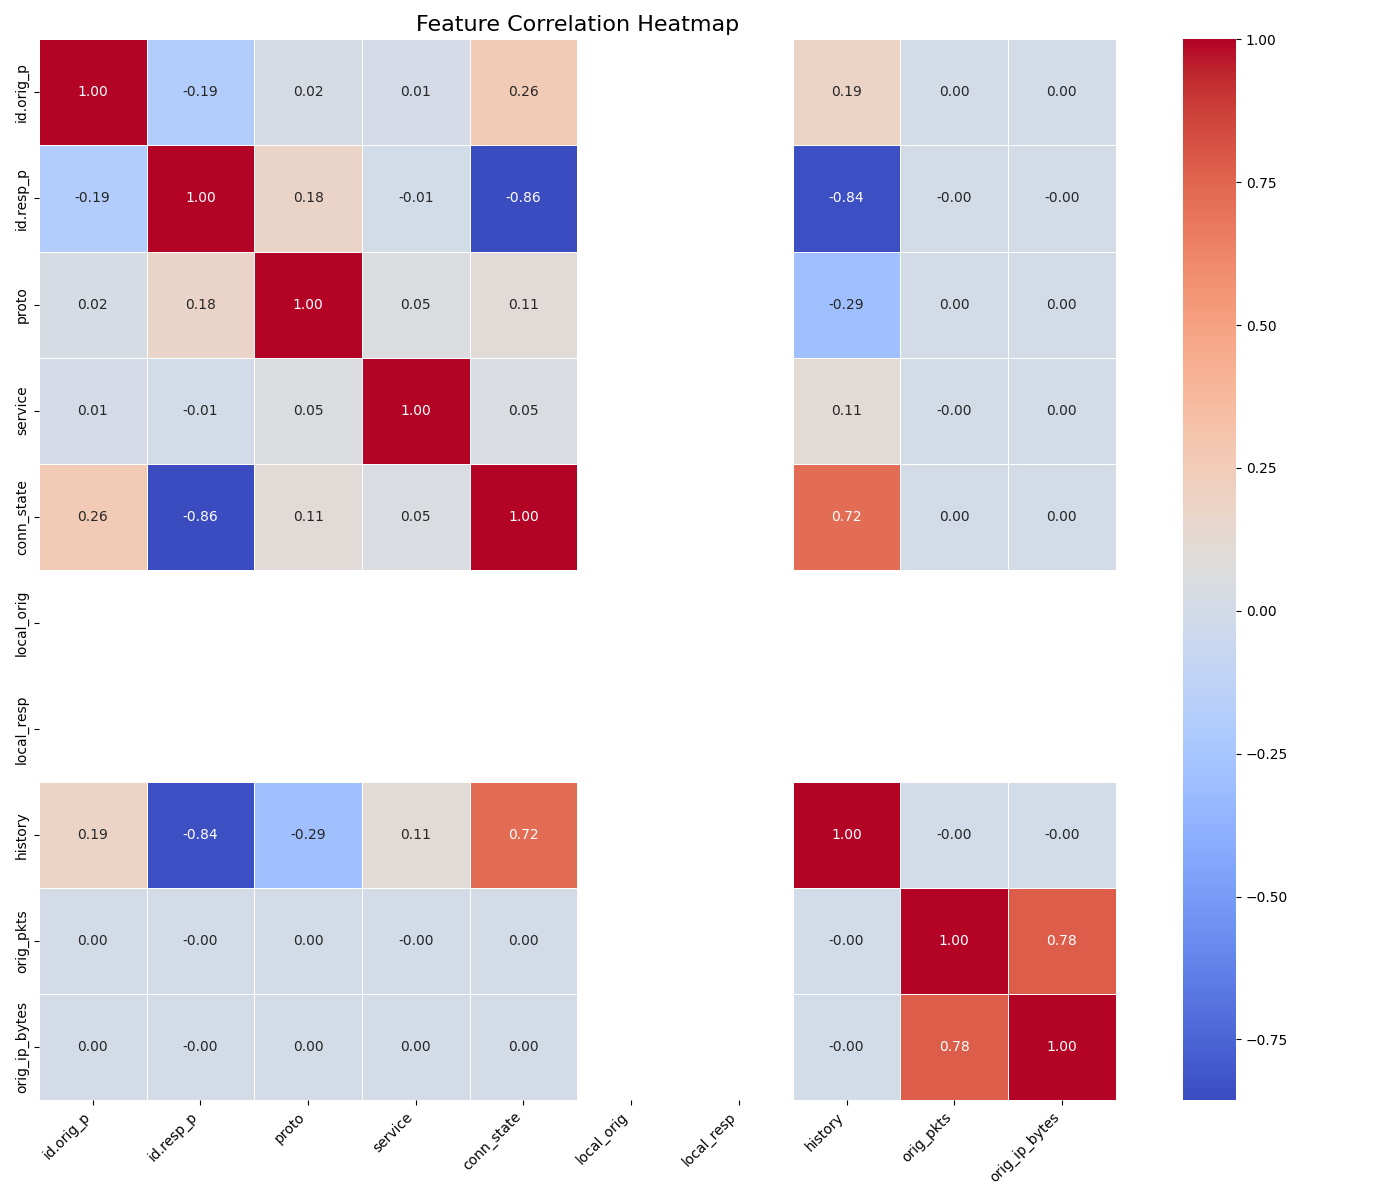
\includegraphics[width=0.8\textwidth]{figures/feature_correlation.png}
    \caption{Correlation heatmap of the top 15 features}
    \label{fig:correlation_heatmap}
\end{figure}
The correlation matrix was computed using the Pearson method, and features with a correlation coefficient greater than 0.9 were considered highly correlated. The features selected for removal were based on their correlation with the target variable (label) and their importance in the model.

\subsection{Recursive Feature Elimination}

After correlation-based filtering, Recursive Feature Elimination with Cross-Validation (RFECV) was applied using a Random Forest estimator. The optimal number of features was determined on the basis of the cross-validated performance:

\begin{table}[h]
\centering
\caption{Feature selection results}
\label{tab:feature_selection}
\begin{tabular}{lcc}
\hline
\textbf{Selection Method} & \textbf{Features Before} & \textbf{Features After} \\
\hline
Correlation-based filtering & 37 & 28 \\
RFECV & 28 & 18 \\
\hline
\end{tabular}
\end{table}

\section{Final Feature Set}

The final set of 18 features used for model training, in order of importance as determined by the Random Forest feature importance scores:

\begin{enumerate}
    \item port\_scan\_score
    \item conn\_rate\_5min
    \item duration (log-transformed)
    \item orig\_bytes (log-transformed)
    \item resp\_bytes (log-transformed)
    \item total\_bytes (log-transformed)
    \item bytes\_per\_pkt\_resp
    \item conn\_state\_S0 (one-hot encoded)
    \item time\_delta\_std
    \item conn\_state\_SF (one-hot encoded)
    \item resp\_pkts (log-transformed)
    \item conn\_state\_REJ (one-hot encoded)
    \item bytes\_ratio
    \item proto\_TCP (one-hot encoded)
    \item hour\_of\_day
    \item is\_scanning\_behavior
    \item proto\_UDP (one-hot encoded)
    \item is\_weekend
\end{enumerate}

This combination of original and derived features provided the best classification performance while maintaining the interpretability and computational efficiency of the model. 
